% =====================================================================
% 附录 AV：氚循环与氚工厂 —— 从增殖到衡算（注明出处）
% ---------------------------------------------------------------------
% 数值唯一来源：tools/calc/appAV_calc.py（只 print，不写文件；输出 tools/calc/appAV_calc.txt）
%   工作点沿用全书 D1：P_fus = 556.5 MW、P_alpha = 111.3 MW、V = 832.2 m^3、
%   R = 6.2 m、a = 2.0 m、n_e0 = 1e20 m^-3、T_e = 9.194 keV；A_wall = 489.532 m^2（与附录 X 一致）
%   核数据：D-T 总释能 17.586 MeV（中子 14.068、alpha 3.518）；6Li(n,alpha)T 释能 4.78 MeV；
%   7Li(n,n'alpha)T 阈值 2.47 MeV；9Be(n,2n) 阈值 1.9 MeV；氚半衰期 12.32 a、平均 beta 能量 5.7 keV
%   声明输入（设计取值）：包层覆盖 0.8、厚 0.5 m、堆积 0.6、密度 2400 kg/m^3；
%   屏蔽有效衰减长度 0.075 m；渗透率有效值 1e-10 mol/(m s Pa^0.5)；提取效率 0.9；
%   燃烧率 0.02；分离因子 1.5 / 1.3；库存 10 kg；衡算精度 1% / 0.5%；氚水限值 1e4 Bq/L
% 单位口径：质量用 g 与 kg，时间用 day 与 a，比活度用 Bq/g，壁负载用 MW/m^2；
%   凡是「设计取值」都在正文里点明是声明输入，不冒充测量值。
% 这一篇讲什么：
%   附录 Z 讲堆的总体账，附录 AJ 讲加料与排灰（含共沉积滞留），附录 AK 讲安全与环境，
%   附录 AP 讲维护与遥操作，附录 AR 讲电源；本附录补上「燃料自己这条链」：
%   增殖（TBR）、提取与分离、渗透与滞留、自持与倍增、衡算与氚水。
% 版权口径：公式与量级口径取自公开发表的经典教材、综述与机构技术文件（见 AV.8 来源表），
%   只保留本书燃料循环场景需要的部分，不复制原书的推导、工艺流程图、代码与图表。
% =====================================================================
\begin{figure}[htbp]
\centering
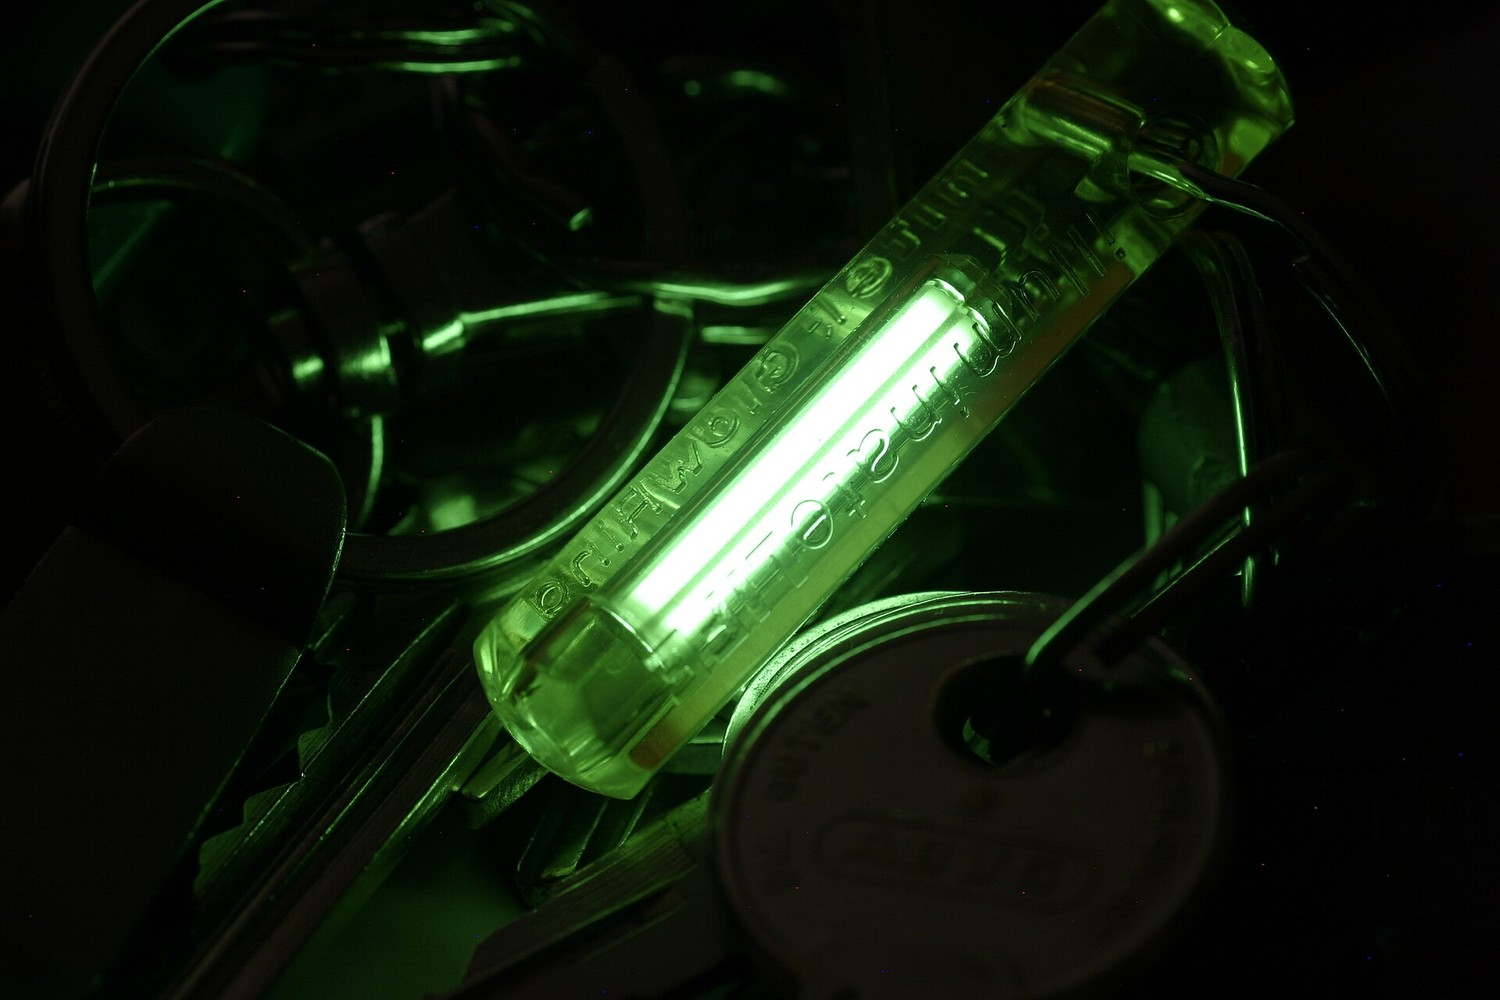
\includegraphics[width=0.72\textwidth]{../figures/tritium_glowring.jpg}
\caption{氚长什么样：自发光的小环。氚的 $\beta$ 衰变（半衰期 12.32 年）激发荧光粉，于是有了这种不需要电池的光源——本章的活度、比活度与剂量换算，说的就是它每秒钟在衰变多少次。}
\label{fig:photo-appav2}
\figsource{Cgommel，CC BY-SA 2.0 de（Wikimedia Commons），链接见 figures/CREDITS.md。}
\end{figure}

\section{三本账：一个反应、两份燃料、三笔账}
\label{sec:app-av-books}

前面每个诊断附录都落在「测出来多少」上；聚变堆却还要回答一个工程问题：烧掉的燃料
怎样补回来。氚在自然界里几乎不存在，必须由中子在中子与锂的反应里现造。于是同一秒钟里
至少有三笔账同时发生：\textbf{烧掉多少}（燃烧）、\textbf{要生回多少}（增殖）、
\textbf{漏掉多少}（渗透与滞留）。把三笔账混成一本，TBR 就会被算错一个百分点——
而一个百分点在氚的问题上就是「自持」与「永远补不回来」的分界。

先算第一本账。D-T 反应一次放出 $17.586\ \mathrm{MeV}$，其中 $14.068\ \mathrm{MeV}$
归中子、$3.518\ \mathrm{MeV}$ 归 alpha 粒子：
\begin{equation}
E_\mathrm{fus}=17.586\ \mathrm{MeV}=2.81759\times10^{-12}\ \mathrm{J},
\label{eq:app-av-rate}
\end{equation}
于是保证 $P_\mathrm{fus}=556.5\ \mathrm{MW}$ 所需要的反应率是
\begin{equation}
R=\frac{P_\mathrm{fus}}{E_\mathrm{fus}}
=\frac{556.5\times10^{6}}{2.81759\times10^{-12}}
=1.97509\times10^{20}\ \mathrm{s^{-1}}.
\label{eq:app-av-burn}
\end{equation}
每一次 D-T 反应烧掉一个氘核与一个氚核，所以 $R$ 同时也是氚的消耗率。中子与 alpha 的
功率份额由式~\eqref{eq:app-av-rate} 直接给出：$79.99545\%$ 与 $20.00455\%$，即
$P_\mathrm{n}=445.175\ \mathrm{MW}$、$P_\alpha=111.325\ \mathrm{MW}$——后者与附录 X、附录 AR
用的 $111.3\ \mathrm{MW}$ 是同一个量，口径一致。

把反应率换成质量要用氚原子质量 $m_\mathrm{T}=5.00827\times10^{-24}\ \mathrm{g}$：
\begin{equation}
\dot m_\mathrm{T}=R\,m_\mathrm{T}
=1.97509\times10^{20}\times5.00827\times10^{-24}
=9.8918\times10^{-4}\ \mathrm{g\,s^{-1}},
\label{eq:app-av-spec}
\end{equation}
也就是每天 $85.4651\ \mathrm{g}$、每年 $31.2161\ \mathrm{kg}$。同法氘每天烧掉
$57.0732\ \mathrm{g}$。工程上更常用的形式是比耗：每 MW 聚变功率每天消耗
$0.153576\ \mathrm{g}$ 氚——记住这个数，它把「功率」与「燃料账单」直接连起来。

\begin{table}[htbp]
\centering
\small
\caption{第一本账：D1 工作点的氚燃烧账（$P_\mathrm{fus}=556.5\ \mathrm{MW}$）}
\label{tab:app-av-books}
\begin{tabular}{p{3.6cm}p{3.4cm}p{4.0cm}p{4.0cm}}
\hline
量 & 值 & 算式 & 口径说明 \\
\hline
单次反应释能 & $17.586\ \mathrm{MeV}$ & 中子 $14.068$ + alpha $3.518$ & 核数据取整到 keV \\
反应率 & $1.97509\times10^{20}\ \mathrm{s^{-1}}$ & $P_\mathrm{fus}/E_\mathrm{fus}$ & 每秒反应数 \\
氚消耗率 & $9.8918\times10^{-4}\ \mathrm{g\,s^{-1}}$ & $R\,m_\mathrm{T}$ & 质量口径 \\
氚日耗 & $85.4651\ \mathrm{g}$ & 乘 $86400$ & 每天 \\
氚年耗 & $31.2161\ \mathrm{kg}$ & 乘 $3.15576\times10^{7}$ & 每年（儒略年） \\
比耗 & $0.153576\ \mathrm{g}$ & 日耗除以 $556.5$ & 每 MW 每天 \\
\hline
\end{tabular}
\end{table}

\begin{tip}{三本账要分开算}{tip-app-av-books}
燃烧、增殖、渗透是三个不同的率：燃烧由 $P_\mathrm{fus}$ 定，增殖由中子经济定，
渗透由分压与壁温定。把它们写成一个「总效率」，就等于放弃了找问题出在哪一格的能力。
\end{tip}

顺带一个自洽性检查：若燃料
按 $n_\mathrm{D}=n_\mathrm{T}=5\times10^{19}\ \mathrm{m^{-3}}$、体积 $V=832.2\ \mathrm{m^{3}}$
填满，则 $R=n_\mathrm{D}n_\mathrm{T}\langle\sigma v\rangle V$ 反推出
$\langle\sigma v\rangle=9.49336\times10^{-23}\ \mathrm{m^{3}\,s^{-1}}$——这正是
$T_\mathrm{e}\approx9.2\ \mathrm{keV}$ 附近的 D-T 反应率量级，说明本工作点自洽。

{\footnotesize
\textbf{出处：}D-T 反应的运动学与反应率系数取自 Bosch \& Hale,
\emph{Nucl. Fusion} \textbf{32}, 611 (1992) 的经典评述。
「三本账」的组织方式参考
Stacey, \emph{Fusion: An Introduction to the Physics and Technology of Magnetic
Confinement Fusion}（2nd ed., Wiley-VCH, 2011）第 11 章与 Dolan 编
\emph{Magnetic Fusion Technology}（Springer, 2013）燃料循环一章的框架，
只保留本书工作点需要的算式。
不复制原书的反应率拟合公式、数据表与算例。
}

\section{增殖：TBR 是「每烧一个氚要生回几个」}
\label{sec:app-av-breeding}

第二本账是增殖。定义上，氚增殖比就是
\begin{equation}
\mathrm{TBR}=\frac{\text{包层里产生的氚}}{\text{等离子体里烧掉的氚}},
\label{eq:app-av-tbr}
\end{equation}
设计值取 $\mathrm{TBR}=1.05$。于是产生率是
\begin{equation}
\dot m_\mathrm{bred}=\mathrm{TBR}\,R\,m_\mathrm{T}
=1.05\times9.8918\times10^{-4}
=1.03864\times10^{-3}\ \mathrm{g\,s^{-1}},
\label{eq:app-av-bred}
\end{equation}
即每天 $89.7384\ \mathrm{g}$（燃烧 $85.4651\ \mathrm{g}$）、每年 $32.7769\ \mathrm{kg}$。
差额只有每天 $2.73301\ \mathrm{g}$——这个小数在 AV.6 会决定倍增时间。

产氚靠两条锂反应。第一条是
\begin{equation}
{}^{6}\mathrm{Li}+\mathrm{n}\rightarrow{}^{3}\mathrm{H}+{}^{4}\mathrm{He}+4.78\ \mathrm{MeV},
\label{eq:app-av-li6}
\end{equation}
它对热中子截面极大，每消耗一个中子换一个氚，所以只靠它 TBR 最多等于 $1$。
第二条是
\begin{equation}
{}^{7}\mathrm{Li}+\mathrm{n}'\rightarrow{}^{3}\mathrm{H}+{}^{4}\mathrm{He}+\mathrm{n}''
-2.47\ \mathrm{MeV}\quad(E_\mathrm{th}=2.47\ \mathrm{MeV}),
\label{eq:app-av-li7}
\end{equation}
它吸能但有阈值以上的中子就能发生，而且\textbf{不消耗中子}：进来的中子出去还是中子。
把 TBR 抬到 $1$ 以上的主力就是它，再往上要靠倍增反应
\begin{equation}
{}^{9}\mathrm{Be}+\mathrm{n}\rightarrow2\,\mathrm{n}'+2\,{}^{4}\mathrm{He}-1.9\ \mathrm{MeV},
\label{eq:app-av-be}
\end{equation}
一个高能中子变两个。

\begin{table}[htbp]
\centering
\small
\caption{增殖反应与中子经济：谁能把 TBR 抬到 1 以上}
\label{tab:app-av-breeding}
\begin{tabular}{p{3.9cm}p{2.2cm}p{2.0cm}p{3.2cm}p{3.4cm}}
\hline
反应 & 能量 & 阈值 & 中子收支 & 作用 \\
\hline
$^{6}$Li(n,$\alpha$)T & 放能 $4.78\ \mathrm{MeV}$ & 无 & 净耗 1 个中子 & 主产氚，TBR 上限 1 \\
$^{7}$Li(n,n'$\alpha$)T & 吸能 $2.47\ \mathrm{MeV}$ & $2.47\ \mathrm{MeV}$ & 中子守恒 & 把 TBR 抬过 1 \\
$^{9}$Be(n,2n) & 吸能 $1.9\ \mathrm{MeV}$ & $1.9\ \mathrm{MeV}$ & 净增 1 个中子 & 倍增剂 \\
\hline
\end{tabular}
\end{table}

产生一个氚要消耗一个 $^{6}$Li，因此锂的消耗可以直接换算：
\begin{equation}
\dot m_{{}^{6}\mathrm{Li}}=\dot m_\mathrm{bred}\frac{M_{{}^{6}\mathrm{Li}}}{M_\mathrm{T}}
=65.3694\ \mathrm{kg\,a^{-1}}.
\label{eq:app-av-limass}
\end{equation}
这个数要按富集度放大：天然锂里 $^{6}$Li 只占 $7.59\%$，取包层富集度 $60\%$ 时
锂元素消耗 $108.949\ \mathrm{kg\,a^{-1}}$；若用天然锂则要 $861.257\ \mathrm{kg\,a^{-1}}$。
折成陶瓷 $\mathrm{Li_4SiO_4}$（摩尔质量 $116.142\ \mathrm{g\,mol^{-1}}$）约
$3163.39\ \mathrm{kg\,a^{-1}}$。

\begin{tip}{TBR 不是「大于 1 就行」}{tip-app-av-tbr}
$1.05$ 与 $1.01$ 都「大于 1」，但前者能自持、后者会被衰变与滞留吃掉全部余量。
判断标准不是 $>1$，而是「净增能否把库存从零补到设计值」——见 AV.6。
\end{tip}

{\footnotesize
\textbf{出处：}锂与铍的中子反应数据取自 IAEA 核数据服务与
Mughabghab, \emph{Atlas of Neutron Resonances}（6th ed., Elsevier, 2018）的口径。
包层增殖比与陶瓷增殖剂的讨论参考 Johnson \& Dean 在
\emph{Fusion Eng. Des.} 系列综述中给出的陶瓷增殖剂材料数据，本书只取质量与摩尔质量换算。
不复制原综述的中子学计算程序、包层几何模型与实验数据表。
}

\section{包层与中子壁负载：中子功率摊在多小的面积上}
\label{sec:app-av-blanket}

中子不带电，离开等离子体后直接打到第一壁与包层上，把 $445.175\ \mathrm{MW}$ 的功率
摊在有限的面积上。第一壁面积沿用附录 X 的几何口径
$A_\mathrm{wall}=4\pi^{2}Ra=489.532\ \mathrm{m^{2}}$，于是平均中子壁负载
\begin{equation}
q_\mathrm{n}=\frac{P_\mathrm{n}}{A_\mathrm{wall}}
=\frac{445.175\times10^{6}}{489.532}
=9.09388\times10^{5}\ \mathrm{W\,m^{-2}}
=0.909388\ \mathrm{MW\,m^{-2}}.
\label{eq:app-av-nwl}
\end{equation}
考虑极向不均匀性取峰值因子 $1.3$，峰值 $1.182205\ \mathrm{MW\,m^{-2}}$。这个量是包层
设计的入口参数：它决定材料的中子损伤速率、氚产生率的体积密度、以及冷却回路要带走的热。

包层要装多少锂，先要算体积：
\begin{equation}
V_\mathrm{blanket}=A_\mathrm{wall}\,f_\mathrm{cov}\,d
=489.532\times0.8\times0.5=195.813\ \mathrm{m^{3}},
\label{eq:app-av-blanket}
\end{equation}
取堆积因子 $0.6$、密度 $2400\ \mathrm{kg\,m^{-3}}$，$\mathrm{Li_4SiO_4}$ 装量
$281.97\ \mathrm{t}$；按 $60\%$ 富集，其中 $^{6}$Li 有 $35048.5\ \mathrm{kg}$。
对照 AV.2 的 $65.3694\ \mathrm{kg\,a^{-1}}$ 消耗，这批装量在不开箱补充的前提下能撑
$536.161\ \mathrm{a}$——所以包层不是「耗材焦虑」，真正的约束是材料损伤与更换周期
（附录 AK 的 50.001 dpa 与附录 AP 的更换周期正是这条约束的两个侧面）。

中子要屏蔽掉。把通量降 $10^{6}$ 倍所需的厚度由指数衰减给出：
\begin{equation}
d=\lambda\ln(10^{6})=0.075\times13.8155=1.03616\ \mathrm{m},
\label{eq:app-av-shield}
\end{equation}
其中 $\lambda=0.075\ \mathrm{m}$ 是钢水混合介质的有效衰减长度（声明取值）。反过来
每米这种介质能把通量压低 $e^{1/\lambda}=617438$ 倍。

\begin{tip}{中子壁负载是面积账，不是功率账}{tip-app-av-nwl}
同样的 $445.175\ \mathrm{MW}$ 中子功率，摊在 $489.532\ \mathrm{m^{2}}$ 上是
$0.909388\ \mathrm{MW\,m^{-2}}$；如果堆的尺寸被人为放大一倍（面积翻倍），壁负载就掉一半。
讨论「壁负载高不高」时，永远要同时说出面积与峰值因子。
\end{tip}

{\footnotesize
\textbf{出处：}中子壁负载与包层厚度的设计口径参考 Abdou 等,
\emph{Fusion Eng. Des.} \textbf{100}, 2 (2015) 与 Federici 等,
\emph{Nucl. Fusion} \textbf{57}, 092002 (2017) 关于 DEMO 包层与第一壁挑战的综述。
屏蔽衰减长度取钢水混合介质的公开量级，作为声明输入写入本节。
不复制原报告的
设计图、材料数据库与屏蔽算例。
}

\begin{table}[htbp]
\centering
\small
\caption{包层与屏蔽：把中子功率、装量与厚度摊开}
\label{tab:app-av-blanket}
\begin{tabular}{p{3.4cm}p{3.4cm}p{3.6cm}p{3.6cm}}
\hline
量 & 值 & 算式 & 说明 \\
\hline
平均中子壁负载 & $0.909388\ \mathrm{MW\,m^{-2}}$ & $P_n/A_\mathrm{wall}$ & 声明面积 \\
峰值（因子 $1.3$） & $1.182205\ \mathrm{MW\,m^{-2}}$ & 乘 $1.3$ & 声明峰值因子 \\
包层体积 & $195.813\ \mathrm{m^{3}}$ & 面积乘覆盖与厚度 & 声明 $80\%$、$0.5$ m \\
$\mathrm{Li_4SiO_4}$ 装量 & $281.97\ \mathrm{t}$ & 乘堆积因子与密度 & 声明 $0.6$、$2400$ \\
其中 $^6$Li & $35048.5\ \mathrm{kg}$ & 按 $60\%$ 富集折算 & 可支撑 $536.161\ \mathrm{a}$ \\
屏蔽厚度（降 $10^{6}$） & $1.03616\ \mathrm{m}$ & $\lambda\ln10^{6}$ & 声明 $\lambda=0.075$ m \\
每米衰减倍数 & $617438$ & $e^{1/\lambda}$ & 对照量级 \\
\hline
\end{tabular}
\end{table}

\section{提取与同位素分离：燃烧率决定了工厂有多大}
\label{sec:app-av-extract}

第三本账之前还有一道关口：增殖出来的氚不在等离子体里，而在包层里。要把燃料送给等离子体，
先要把氚从包层里提出来；要从等离子体排气流里把没烧掉的氚收回来。这两件事都由一个参数
放大——燃烧率 $f_\mathrm{b}$。D1 工作点按 $f_\mathrm{b}=0.02$ 取（声明取值），于是一定要注入
\begin{equation}
\dot m_\mathrm{inj}=\frac{\dot m_\mathrm{T}}{f_\mathrm{b}}
=\frac{85.4651}{0.02}
=4273.26\ \mathrm{g\,day^{-1}}=4.27326\ \mathrm{kg\,day^{-1}},
\label{eq:app-av-inject}
\end{equation}
也就是每年 $1.56081\ \mathrm{t}$ 的氚要通过工厂——是燃烧量的 $50$ 倍，其中 $98\%$ 必须回收。
这就是「氚工厂」的规模从哪来的：不是由堆功率单独决定，而是由功率乘上 $1/f_\mathrm{b}$ 决定。
燃烧率提高一倍，工厂规模减半；这也是为什么先进位形与高约束模式的研究会直接改善燃料循环经济性。

提取效率 $\eta_\mathrm{ext}$ 直接乘在增殖比上。如果每一轮循环只能取出 $90\%$（声明取值），
那么为了补回烧掉的那一份，增殖比至少要
\begin{equation}
\mathrm{TBR}_\mathrm{min}=\frac{1}{\eta_\mathrm{ext}}=\frac{1}{0.9}=1.11111,
\label{eq:app-av-tbrmin}
\end{equation}
这已经远高于 $1$。再加上衰变损失（AV.6），真正的及格线还会更高。

回收之后要分离同位素：排气流里是 D、T 与 He 的混合物，要用低温蒸馏把氚富集回
燃料所需的份额。理论板数由分离因子 $\alpha$ 决定：
\begin{equation}
N=\frac{\ln\left[\dfrac{x_\mathrm{P}}{1-x_\mathrm{P}}\Big/\dfrac{x_\mathrm{F}}{1-x_\mathrm{F}}\right]}{\ln\alpha},
\label{eq:app-av-stage}
\end{equation}
把进料 $x_\mathrm{F}=0.5$ 提到产品 $x_\mathrm{P}=0.9$，取 $\alpha=1.5$ 得 $N=5.41902$ 块理论板；
若分离因子只有 $\alpha=1.3$（分离因子差 $1.154$ 倍），板数涨到 $8.37471$ 块，是前者的
$1.54543$ 倍。要提到 $x=0.99$，$\alpha=1.5$ 下需要 $11.333$ 块。这解释了为什么
同位素分离系统的体积与投资对分离因子极其敏感。

\begin{table}[htbp]
\centering
\small
\caption{提取与分离：由燃烧率与分离因子决定的工厂规模}
\label{tab:app-av-extract}
\begin{tabular}{p{3.6cm}p{3.2cm}p{3.6cm}p{4.2cm}}
\hline
量 & 值 & 算式 & 口径 \\
\hline
注入率 & $4.27326\ \mathrm{kg\,day^{-1}}$ & 日耗除以 $f_\mathrm{b}=0.02$ & 声明燃烧率 \\
年通过量 & $1.56081\ \mathrm{t}$ & 乘 $365.25$ & 工厂处理量 \\
未燃份额 & $98\%$ & $1-f_\mathrm{b}$ & 必须回收 \\
提取效率 & $90\%$ & 声明取值 & 每轮循环 \\
$\mathrm{TBR}_\mathrm{min}$ & $1.11111$ & $1/\eta_\mathrm{ext}$ & 只补燃烧、不含衰变 \\
理论板数 & $5.41902$ & $\alpha=1.5$，$x:0.5\rightarrow0.9$ & 低温蒸馏 \\
理论板数 & $8.37471$ & $\alpha=1.3$ 同工况 & 敏感度对照 \\
\hline
\end{tabular}
\end{table}

\begin{tip}{提取效率是乘在 TBR 上的}{tip-app-av-extract}
TBR 与提取效率不是「两个独立的 90\%」：没提出来的氚等于没增殖。写设计指标时要把
$\eta_\mathrm{ext}$ 放进 $\mathrm{TBR}_\mathrm{min}$，而不是留在「以后优化」的清单里。
\end{tip}

{\footnotesize
\textbf{出处：}低温蒸馏分离氢同位素的理论板数口径参考 Cristescu 等在国际热核聚变实验堆
同位素分离系统设计文献中的写法（\emph{Fusion Sci. Technol.} 系列）。
ITER 氚工厂的总体流程与规模参考 Glugla 等，\emph{Fusion Eng. Des.} \textbf{82}, 472 (2007)。
本书只借用「板数由分离因子与进料/产品份额决定」这一个关系，不复制原文献的流程框图、
塔板结构与运行参数。
}

\section{渗透与滞留：库存不是一个数，是一条链}
\label{sec:app-av-permeation}

氚是氢的同位素，会穿过金属。渗透的问题不是「有没有」，而是「多快」：高温下氢同位素
在金属中的渗透通量遵守平方根定律
\begin{equation}
J=\frac{\Phi_\mathrm{eff}\sqrt{p_\mathrm{T}}}{d},
\label{eq:app-av-perm}
\end{equation}
其中 $\Phi_\mathrm{eff}$ 是有效渗透率、$p_\mathrm{T}$ 是氚分压、$d$ 是壁厚。
取声明值 $\Phi_\mathrm{eff}=10^{-10}\ \mathrm{mol\,m^{-1}\,s^{-1}\,Pa^{-0.5}}$、
$p_\mathrm{T}=10\ \mathrm{Pa}$、$d=2\ \mathrm{mm}$，得
$J=1.58114\times10^{-7}\ \mathrm{mol\,m^{-2}\,s^{-1}}$，也就是
$0.0412024\ \mathrm{g\,m^{-2}\,day^{-1}}$。

把通量乘上热表面面积 $A_\mathrm{hot}=500\ \mathrm{m^{2}}$ 与渗透降低因子
$\mathrm{PRF}=100$（声明取值，来自氧化层或镀层），年渗透量
\begin{equation}
\dot m_\mathrm{perm}=\frac{J\,A_\mathrm{hot}\,M_\mathrm{T}\times3.15576\times10^{7}}{\mathrm{PRF}}
=75.2458\ \mathrm{g\,a^{-1}},
\label{eq:app-av-decay}
\end{equation}
占燃烧量的 $0.241048\%$。不加壁垒则是 $7524.58\ \mathrm{g\,a^{-1}}$——两者相差正好
$\mathrm{PRF}$ 倍。注意这里的平方根：把分压提高 $100$ 倍，通量只涨 $10$ 倍；
把壁厚减半，通量才翻倍。所以渗透控制的抓手是「挡」（壁垒）与「减面积」，不是「抽」。

\begin{table}[htbp]
\centering
\small
\caption{渗透与滞留：每一格都是一条可检查的乘法链}
\label{tab:app-av-permeation}
\begin{tabular}{p{3.4cm}p{3.4cm}p{3.6cm}p{4.2cm}}
\hline
项 & 值 & 算式 & 说明 \\
\hline
渗透通量 & $1.58114\times10^{-7}\ \mathrm{mol\,m^{-2}\,s^{-1}}$ & $\Phi\sqrt{p}/d$ & 平方根定律 \\
质量通量 & $0.0412024\ \mathrm{g\,m^{-2}\,d^{-1}}$ & 乘 $M_\mathrm{T}$ 与 $86400$ & 每平方米每天 \\
年渗透（有壁垒） & $75.2458\ \mathrm{g}$ & 乘 $500\ \mathrm{m^{2}}$ 除以 $100$ & 声明 PRF \\
年渗透（无壁垒） & $7524.58\ \mathrm{g}$ & 同上、PRF 取 $1$ & 对照 \\
占燃烧量 & $0.241048\%$ & 除以 $31.2161\ \mathrm{kg}$ & 相对份额 \\
共沉积滞留 & $603.647\ \mathrm{g}$ & 附录 AJ 口径 & 库存的 $6.03647\%$ \\
\hline
\end{tabular}
\end{table}

渗透只是「漏」，还有「存」：氚会被共沉积层捕获（附录 AJ 给出 $603.647\ \mathrm{g}$，
相当于 $10\ \mathrm{kg}$ 库存的 $6.03647\%$），也会在管路、泵与冷阱里以滞留形式累积。
最后才轮到库存本身，而库存有它自己的时钟：氚的半衰期 $12.32\ \mathrm{a}$ 给出
$\lambda=1.78283\times10^{-9}\ \mathrm{s^{-1}}$。$10\ \mathrm{kg}$ 库存对应
$1.9967\times10^{27}$ 个氚原子，活度 $3.55978\times10^{18}\ \mathrm{Bq}$
（$3.55978\times10^{6}\ \mathrm{TBq}$），衰变热按平均 beta 能量 $5.7\ \mathrm{keV}$ 计
$3250.94\ \mathrm{W}=3.25094\ \mathrm{kW}$。每天衰变掉 $1.54025\ \mathrm{g}$，
相当于燃烧量的 $1.8022\%$——这个数看着小，但它是每天都要补的。

\begin{tip}{渗透率是平方根定律，不是线性定律}{tip-app-av-permeation}
「把分压提高一倍，渗透翻倍」是错的：$\sqrt{2}=1.41421$。反过来说，靠降低分压来治渗透
收益很小，把 $\Phi_\mathrm{eff}$ 压低两个量级才是正解。
\end{tip}

{\footnotesize
\textbf{出处：}氢同位素在金属中的渗透与渗透降低因子参考 Hollenberg 等,
\emph{Fusion Eng. Des.} \textbf{28}, 190 (1995) 关于氚/氢渗透壁垒的经典综述。
共沉积滞留口径与附录 AJ 一致。本书只取「平方根定律 + PRF 的乘法链」这一层，
不复制原综述的渗透率数据库、镀层工艺与实验装置图。
}

\section{自持：TBR 的及格线在哪里}
\label{sec:app-av-selfsuff}

现在把三本账合起来。库存要维持，必须让产生率不小于「燃烧 + 衰变 + 提取损失」。
先只看前两项：最小自持增殖比
\begin{equation}
\mathrm{TBR}_\mathrm{min}=\frac{\dot m_\mathrm{T}+\dot m_\mathrm{decay}}{\dot m_\mathrm{T}}
=\frac{85.4651+1.54025}{85.4651}=1.01802,
\label{eq:app-av-tbrmin2}
\end{equation}
再把提取效率 $0.9$ 除进去，得到 $1.13114$——这才是真正的及格线。也就是说，
$\mathrm{TBR}=1.05$ 的设计值并不宽裕，它把 $1.01802$ 与 $1.13114$ 之间的余量全押在
「提取效率做得到 $90\%$」上。

净增与倍增时间是同一件事的两种说法。定义
\begin{equation}
\dot m_\mathrm{net}=\mathrm{TBR}\,\dot m_\mathrm{T}-\dot m_\mathrm{T}-\dot m_\mathrm{decay},
\label{eq:app-av-net}
\end{equation}
库存 $10\ \mathrm{kg}$ 从零补到设计值的倍增时间是 $t_\mathrm{d}=m_\mathrm{inv}/\dot m_\mathrm{net}$。
四个 TBR 的结果列在表~\ref{tab:app-av-selfsuff}：$1.02$ 要 $161.952\ \mathrm{a}$（工程上等于
永远补不回来），$1.05$ 要 $10.0177\ \mathrm{a}$，$1.08$ 要 $5.16872\ \mathrm{a}$，
$1.10$ 只要 $3.90772\ \mathrm{a}$。

\begin{table}[htbp]
\centering
\small
\caption{自持：净增、倍增时间与「及格线」的距离（库存 $10\ \mathrm{kg}$）}
\label{tab:app-av-selfsuff}
\begin{tabular}{p{2.4cm}p{3.0cm}p{3.4cm}p{5.2cm}}
\hline
TBR & 净增 & 倍增时间 & 说明 \\
\hline
$1.02$ & $0.169053\ \mathrm{g\,day^{-1}}$ & $161.952\ \mathrm{a}$ & 只比及格线高一点，工程上不可用 \\
$1.05$ & $2.73301\ \mathrm{g\,day^{-1}}$ & $10.0177\ \mathrm{a}$ & D1 设计值 \\
$1.08$ & $5.29696\ \mathrm{g\,day^{-1}}$ & $5.16872\ \mathrm{a}$ & 中等余量 \\
$1.10$ & $7.00626\ \mathrm{g\,day^{-1}}$ & $3.90772\ \mathrm{a}$ & 余量充足 \\
\hline
\end{tabular}
\end{table}

库存还有一个时间尺度：工厂把库存循环一遍要多久。按注入量 $4.27326\ \mathrm{kg\,day^{-1}}$，
$10\ \mathrm{kg}$ 的循环时间是
\begin{equation}
t_\mathrm{cyc}=\frac{m_\mathrm{inv}}{\dot m_\mathrm{inj}}
=\frac{10}{4.27326}=2.34014\ \mathrm{day},
\label{eq:app-av-cycle}
\end{equation}
循环一圈衰变掉的份额只有 $0.0360402\%$。循环时间越短，滞留与衰变损失越小；
但它不能无限缩短——工厂的处理能力与库存都要钱。

\begin{tip}{倍增时间不是「堆的寿命」}{tip-app-av-doubling}
倍增时间是「用净增把库存从零补到设计值」需要多久，它是自持能力的度量，不是运行寿命。
$161.952\ \mathrm{a}$ 的含义不是「能跑 162 年」，而是「一直没有足够燃料启动」。
\end{tip}

{\footnotesize
\textbf{出处：}氚自持与倍增时间的分析框架参考 ITER 技术基础文件
（\emph{ITER Technical Basis}, IAEA, 2002）关于氚库存与增殖要求的讨论，
以及 Stacey（2011）第 11 章的自持判据。本节所有数字由
\texttt{tools/\allowbreak{}calc/\allowbreak{}appAV\_calc.py} 按本书工作点复算。
不复制原文件的库存限值表与增殖包层方案。
\section{衡算、安全与环境：百分之零点五的精度意味着什么}
\label{sec:app-av-account}
}

氚是会「跑」的：它会渗透、会被滞留、会衰变，而每一种损失都很难直接称重。燃料循环能不能
闭合，最后靠的不是流量计，而是衡算——用「进去的减出来的」来推断「还剩多少」。
库存 $10\ \mathrm{kg}$ 上做 $1\%$ 的衡算，不确定度就是 $100\ \mathrm{g}$，相当于
$1.17007$ 天的燃烧量；要做到 $0.5\%$，不确定度压到 $50\ \mathrm{g}$，即
$0.585034$ 天的燃烧量。反过来说，若要求衡算误差不超过「一天烧掉的量」，
精度必须优于 $0.854651\%$。这就是为什么氚衡算系统的指标是「天」而不是「百分比」：
一天的量是可以对照流量计核对的，百分比的绝对值不行。

\begin{table}[htbp]
\centering
\small
\caption{衡算与安全：把百分比翻译成克、天与立方米}
\label{tab:app-av-account}
\begin{tabular}{p{3.4cm}p{3.4cm}p{3.8cm}p{3.6cm}}
\hline
量 & 值 & 算式 & 说明 \\
\hline
$1\%$ 衡算 & $100\ \mathrm{g}$ & $10\ \mathrm{kg}\times0.01$ & $1.17007$ 天燃烧量 \\
$0.5\%$ 衡算 & $50\ \mathrm{g}$ & 同上 & $0.585034$ 天 \\
要求 $\le1$ 天 & $0.854651\%$ & 燃烧量除以库存 & 精度上限 \\
氚比活度 & $3.55978\times10^{14}\ \mathrm{Bq\,g^{-1}}$ & 活度除以库存 & 纯氚 \\
氚水比活度 & $5.33967\times10^{13}\ \mathrm{Bq\,g^{-1}}$ & 每克 HTO 含 $0.334327$ g 氚 & HTO \\
稀释 $1\ \mathrm{g}$ HTO & $5.33967\times10^{6}\ \mathrm{m^{3}}$ & 除以 $10^{4}\ \mathrm{Bq\,L^{-1}}$ & 饮用水限值 \\
稀释 $1\ \mathrm{g}$ 氚 & $3.55978\times10^{7}\ \mathrm{m^{3}}$ & 同上、折成 HTO & 对照 \\
库存天数 & $117.007$ & $10\ \mathrm{kg}$ 除以日耗 & 无加料可撑多久 \\
\hline
\end{tabular}
\end{table}

把库存全放出去会怎样？$10\ \mathrm{kg}$ 的总活度是 $3.55978\times10^{18}\ \mathrm{Bq}$，
全部以 HTO 形式释放要 $3.55978\times10^{11}\ \mathrm{m^{3}}$ 的水才稀释到限值——
这个体积是荒谬的，所以氚安全从来不是「稀释达标」，而是「不让它出来」：多重包容、
负压手套箱、催化氧化与分子筛捕集。衡算的真正意义也在这里：它是包容失效的探针。
库存天数 $117.007$ 天则给出另一个直觉——不加料的话，$10\ \mathrm{kg}$ 库存撑不到四个月。

\begin{tip}{衡算精度是时间尺度，不是百分数}{tip-app-av-account}
把 $0.5\%$ 说成「精度要求」很抽象，说成「$0.585034$ 天的燃烧量」就立刻可操作：
它与加料系统的日流量同量级，因此可以被独立核对。
\end{tip}

{\footnotesize
\textbf{出处：}氚衡算与氚安全的分级参照 ITER 氚安全与衡算体系文件
（\emph{ITER Tritium Safety} 系列, 2018）与 IAEA 氚环境排放限值口径。
比活度与稀释体积由 \texttt{tools/\allowbreak{}calc/\allowbreak{}appAV\_calc.py} 按本书工作点复算。
本书只借用「衡算误差折成天数」这一判据，不复制原文件的限值表、监测系统方案与事故分析。
}

\section{估算练习}
\label{sec:app-av-problems}

以下题目都可以用本章的算式手算。答案在题后给出，保留六位有效数字；
建议先自己算，再对照解答核对口径。

\textbf{练习 1}
另一台装置的聚变功率为 $800\ \mathrm{MW}$。按本章的 $E_\mathrm{fus}=17.586\ \mathrm{MeV}$，
求氚的日消耗、年消耗与单位功率比耗。

\textbf{解答 1}
$R=P/E_\mathrm{fus}=2.83930\times10^{20}\ \mathrm{s^{-1}}$，日耗
$122.861\ \mathrm{g\,day^{-1}}$、年耗 $44.875\ \mathrm{kg\,a^{-1}}$，
比耗 $0.153576\ \mathrm{g\,(MW\,day)^{-1}}$。

\textbf{练习 2}
取 $\mathrm{TBR}=1.08$、库存 $8\ \mathrm{kg}$，求净增与倍增时间（衰变按库存比例折算）。

\textbf{解答 2}
净增 $5.60501\ \mathrm{g\,day^{-1}}$，倍增时间 $3.90772\ \mathrm{a}$。

\textbf{练习 3}
若提取效率只有 $85\%$，最小自持增殖比是多少？

\textbf{解答 3}
$\mathrm{TBR}_\mathrm{min}=(1+\dot m_\mathrm{decay}/\dot m_\mathrm{T})/\eta
=1.01802/0.85=1.19767$。

\textbf{练习 4}
把渗透降低因子从 $100$ 提高到 $200$（其余不变），年渗透量变成多少？占燃烧量多少？

\textbf{解答 4}
$37.6229\ \mathrm{g\,a^{-1}}$，占燃烧量 $0.120524\%$（正好减半）。

\textbf{练习 5}
用低温蒸馏把氚份额从 $0.5$ 提到 $0.95$，比较 $\alpha=1.3$ 与 $\alpha=1.5$ 的理论板数。

\textbf{解答 5}
$\alpha=1.3$ 需 $11.2227$ 板，$\alpha=1.5$ 需 $7.26188$ 板，两者相差 $1.54543$ 倍。

\textbf{练习 6}
$10\ \mathrm{kg}$ 库存、衡算精度 $0.5\%$，折成多少克、多少天的燃烧量？

\textbf{解答 6}
$50\ \mathrm{g}$，相当于 $0.585034$ 天的燃烧量。

\section{来源、分级与版权说明}
\label{sec:app-av-source}

\begingroup\small
本附录的定位是「燃料循环的账本」：它把氚的耗、生、存、取、算五件事写成可以复算的
乘法链，并显式区分哪些量来自核数据、哪些量是本书声明输入。全书所有数字由
\texttt{tools/\allowbreak{}calc/\allowbreak{}appAV\_calc.py} 按 D1 工作点复算，正文不引用任何未在本附录出现的数值。

\textbf{借鉴来源与边界}（分级：核心口径来自 A 类，材料与工程数据来自 B 类）：
\begin{itemize}
  \item \textbf{Freidberg, \emph{Plasma Physics and Fusion Energy}（Cambridge, 2007）}
  的燃料循环与功率平衡框架：本书借用「反应率—消耗—比耗」的推导结构（AV.1），
  不复制原书习题与图表。
  \item \textbf{Wesson, \emph{Tokamaks}（4th ed., Oxford, 2011）}关于 D-T 反应与
  中子功率分配的核数据口径（AV.1）。
  \item \textbf{Stacey, \emph{Fusion Plasma Physics}（2nd ed., Wiley-VCH, 2011）}
  第 11 章的增殖比与自持判据（AV.2、AV.6）。
  \item \textbf{Dolan 编, \emph{Magnetic Fusion Technology}（Springer, 2013）}
  燃料循环一章的提取、分离与工厂规模讨论（AV.4）。
  \item \textbf{Glugla 等, \emph{Fusion Eng. Des.} \textbf{82}, 472 (2007)}：
  ITER 氚工厂流程与规模的公开综述（AV.4、AV.5）。
  \item \textbf{Hollenberg 等, \emph{Fusion Eng. Des.} \textbf{28}, 190 (1995)}：
  氢同位素渗透与渗透降低因子的经典综述（AV.5）。
  \item \textbf{\emph{ITER Technical Basis}（IAEA, 2002）}与
  \textbf{\emph{ITER Tritium Safety}（2018）}：自持要求、库存限值与衡算分级（AV.6、AV.7）。
\end{itemize}

\textbf{不复制声明}：以上来源仅用于核对公式形式、术语与数量级；本附录的全部算式、
表格、数值与练习均为本书按 D1 工作点独立复算的结果，不复制任何原文献的段落、
数据表、图、习题或代码。凡属设计取值的量（燃烧率、提取效率、分离因子、渗透率有效值、
包层参数、库存与衡算精度）均在正文中显式标注为「声明输入」，读者可以替换后重算。

\textbf{本附录不做什么}：不给中子输运计算（那需要蒙卡程序与三维几何），
不给氚工厂的工艺流程图与设备尺寸设计，不给安全分析（事故序列与后果评价），
也不给氚在环境中的迁移模型——这些分别属于中子学、化工与安全分析专著的范围。
\endgroup
